\chapter{Método propuesto}

En el capítulo 3 se describieron los principales retos del perfilado de autor y las principales características de los métodos existentes para el aumento de datos en la clasificación de textos. Observando las características de los métodos de aumento de datos existentes, en este capítulo se describen los métodos propuestos para realizar el aumento de datos para tareas relacionadas al perfilado de autor. 

Como se mostró en el capítulo anterior, existen numerosas técnicas de aumento de datos sin embargo no todas son generalizables o escalables, además de que en el caso de perfilado de autor se desea conservar tanto el estilo como el contenido de un texto. De ahí que la mejor forma de realizar el aumento de datos en esta tarea es mediante el parafraseo humano, pero debido a su costo, no siempre es posible. Sin embargo nos podemos apoyar de técnicas automáticas para aproximarse al parafraseo \citep{androutsopoulos2010survey}. 

El aumento de datos propuesto busca aproximarse al parafraseo de las frases originales y con ellas incrementar el conjunto original. Los métodos desarrollados en este trabajo tienen dos pasos generales que se describen a continuación: 

\begin{enumerate}
    \item \textbf{Selección de palabras a reemplazar}: El primer paso consiste en identificar el subconjunto de palabras a reemplazar. Dos criterios son relevantes en esta etapa: (i) la importancia de la palabra en la estructura de la frase, es decir, no se tiene el mismo efecto si se  reemplaza una palabra de contenido que una palabra funcional; (ii) la cantidad de palabras a reemplazar, dado que se desea conservar la misma interpretación de la frase original el número de reemplazos deberá controlarse.  
    \item \textbf{Reemplazo de palabras seleccionadas}: Una vez determinado el subconjunto de palabras a reemplazar, se deberán identificar nuevas palabras que no alteren significativamente el sentido de la frase original. Para ello se recurre a un recurso externo, tal como un tesauro, un diccionario, o incluso a modelos distribucionales de vectores de palabras.
    Una vez identificadas las palabras sustitutas se reconstruye la secuencia manteniendo el orden original para formar la nueva secuencia aumentada. 
\end{enumerate}





%\begin{enumerate}
%    \item \textbf{Texto original}: La entrada es una secuencia de palabras $S$ de tamaño $n$, la cual se divide en tokens mediante un separador (p. e. puede ser un espacio o una expresión regular).
%    \item \textbf{Selección de palabras a reemplazar}: mediante algún criterio de selección se identifica un subconjunto de tokens $S_1$ del conjunto $S$ de tamaño $r$. 
%    \item \textbf{Identificación de palabras sustitutas}: Una vez determinado el subconjunto $S_1$ de palabras a reemplazar, se crean los conjuntos $R_{w_i}$ con posibles palabras sustitutas para cada palabra $w_i \in S_1$. Para ello se utiliza un recurso externo. Este recurso puede ser un tesauro, un diccionario o modelos pre-entrenados de vectores de palabras.
%    \item \textbf{Reemplazo}: Mediante algún criterio de similitud buscamos la palabra $w'_i$ que reemplazará a la palabra $w_i$ para cada conjunto $R_{w_i}$. Una vez identificadas todas las palabras sustitutas se reconstruye la secuencia manteniendo el orden original para formar la nueva secuencia aumentada $S_{aug}$. 
%    \item \textbf{Reemplazo}: La última fase reemplaza las palabras seleccionadas por las palabras candidatas encontradas en el recurso externo.
%\end{enumerate}
 
%\begin{figure}
    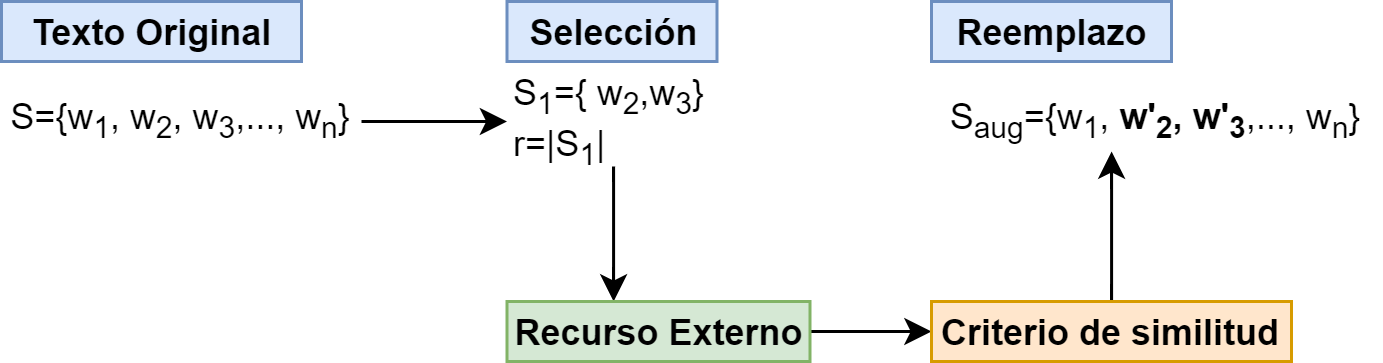
\includegraphics[width=\textwidth]{sections/figures/word_level.png}
    \caption{Aumento de datos a nivel palabra mediante reemplazo de sinónimos}
    \label{fig:aumento}
\end{figure}

%El problema principal radica en como realizar la selección de palabras, de tal forma que se conserve tanto el estilo como el contenido de la secuencia original $S$. Para esto se proponen diferentes métodos enfocados a distintos aspectos en el proceso de selección y reemplazo.


\section{Selección de palabras a reemplazar}

El primer punto bajo este proceso es el cálculo del número de palabras a reemplazar. Para ello, se retomó el criterio presentado en \citep{zhang2015character}. El número de palabras a reemplazar $r$ se selecciona realizando un muestreo aleatorio de una distribución de probabilidad geométrica. 

Una función de probabilidad geométrica es la función de probabilidad del número $X$ del ensayo de Bernoulli de obtener éxito, soportado en el conjunto de los números naturales. Una distribución geométrica da la probabilidad de que la primera ocurrencia de éxito requiere de $k$ ensayos independientes, cada uno con una probabilidad de éxito $p$. Si la probabilidad de éxito de cada ensayo es $p$, entonces la probabilidad de que en el $k$-ésimo ensayo, de $k$ ensayos, sea el primer éxito es representada en la ecuación \ref{eq:geom}.

\begin{equation} \label{eq:geom}
    Pr(X=k)=(1-p)^{k-1}p
\end{equation}

Por lo tanto la aleatoriedad del número $r$ es controlada mediante la modificación del parámetro $p$ como se representa en figura \ref{fig:geom}. Como puede verse en dicha figura, mientras menor sea el valor de $p$ se modificará un mayor número de palabras, agregando una mayor diversidad  y consecuentemente incrementando la probabilidad de alterar el significado original. 
\begin{figure}[ht]
    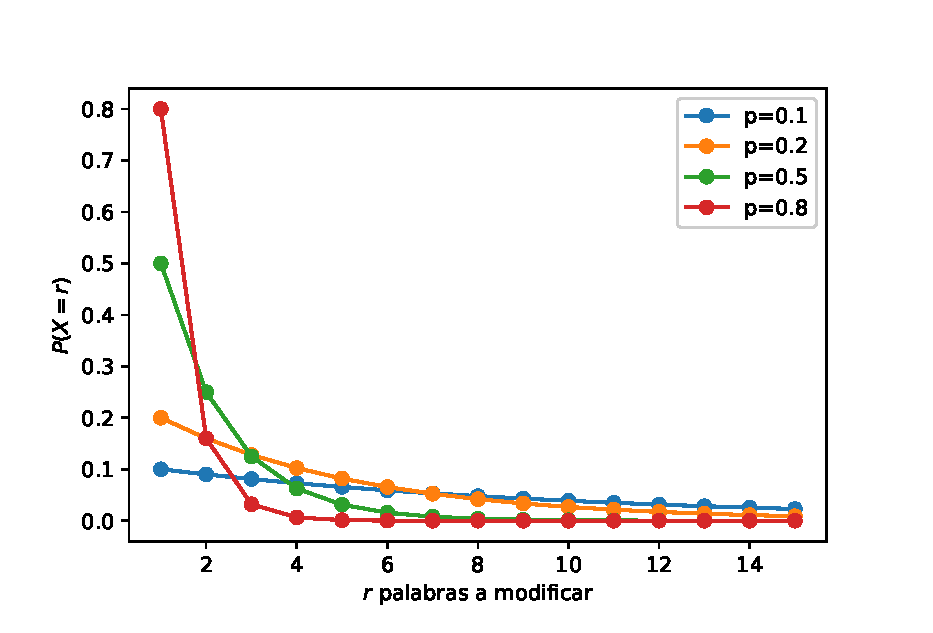
\includegraphics[width=\textwidth]{sections/figures/geometric_pmf.eps}
    \caption{Función de masa para la distribución geométrica con diferentes valores de probabilidad.}
    \label{fig:geom}
\end{figure}

\subsection{Etiquetado de partes de la oración}

El proceso de selección debe cuidar la modificación de ciertas partes de la oración para, por un lado, evitar perder la interpretación original, y por otro intentar conservar el estilo de la frase original. Por tal motivo, cada frase es etiquetada asignando a cada palabra su etiqueta POS (\textit{part of speech}) correspondiente. La tabla \ref{table:pos} muestra un ejemplo del tipo de etiquetado aplicado. Gracias al etiquetado las palabras a reemplazar solo son aquellas que están más fuertemente asociadas al contenido de la frase, es decir, solo se seleccionan aquellas palabras con funciones gramaticales de: sustantivo, adjetivo, verbo y/o adverbio.


\begin{table}[h]
\caption{Ejemplo de etiquetado de partes de la oración.} \label{table:pos}
\begin{center}
\begin{tabular}{lllllll}
\hline
\textbf{Secuencia} & \textit{I} & \textit{am} & \textit{running} & \textit{out} & \textit{of} & \textit{ideas} \\ \hline
Etiqueta           & PRP        & VBP         & VBG              & IN           & IN          & NNS            \\ \hline
Equivalencia       & Pronombre  & Verbo       & Verbo            & Preposición  & Preposición & Sustantivo     \\ \hline
\end{tabular}
\end{center}
\end{table}

\subsection{Exclusión de palabras importantes}

%Agregar porque se necesitan excluir
%Después de seleccionar el valor de $r$ palabras a reemplazar lo siguiente es seleccionar que palabras seran reemplazadas. Con el objetivo de mantener la estructura del texto se proponen una seria de reglas o métodos, el primer paso es excluir las palabras de paro pertenecientes al idioma del conjunto de texto a aumentar.

% \subsubsection{Chi cuadrada}
Además de las palabras funcionales también es deseable mantener palabras que aportan información para la tarea de clasificación que se desea realizar, por lo tanto la primera propuesta consiste en evitar seleccionar, entre las palabras a reemplazar, aquellas  palabras dependientes a la clase del documento. 

Para este proceso recurrimos a la técnica de selección de características conocida como prueba de independencia $\chi^2$ (Chi cuadrada). En estadística, la prueba $\chi^2$ es aplicada para comprobar la independencia de dos eventos, donde los eventos $A$ y $B$ son definidos a ser independientes si  $P(AB)= P(A)P(B)$ o, equivalente, $P(A|B)=P(A)$ y $P(B|A)=P(B)$. En la selección de características para la clasificación de textos, los dos eventos son: \textit{ocurrencia del término} y \textit{ocurrencia de la clase}. Posteriormente se ordenan los términos de mayor a menor respecto a la ecuación \ref{eq:chi2}.

\begin{equation}
    \label{eq:chi2}
    \chi^2(D, t, c)= \sum_{e_t \in {0,1} }^{} \sum_{e_c \in {0,1} }^{} \frac{(N_{e_t e_c} - E _{e_t e_c})^2}{E_{e_t e_c}}
\end{equation}

El término $e_t$ indica la ausencia o presencia del término $t$ en el documento, similarmente el término $e_c$ indica si el documento se encuentra en la clase $c$. $N$ es la frecuencia observada en $D$ y $E$ es la frecuencia esperada. $\chi^2$ mide por cuanto los conteos esperados $E$ y los conteos observados $N$ se desvían de cada uno. Un valor alto de $\chi^2$ indica que la hipótesis de independencia, la cual implica que los conteos esperados y observados son similares, es incorrecta. Si los dos eventos son dependientes, entonces la ocurrencia del término hace la ocurrencia de la clase más probable (o menos probable), entonces el término debería ser seleccionado como relevante.

A través de este método se identifican todas aquellas palabras dependientes de la clase, y por ende, de relevancia para la tarea de clasificación. Dada la importancia de estas palabras se evitará reemplazarlas, excluyéndolas del proceso de selección de palabras a reemplazar.

\section{Reemplazo de palabras seleccionadas}

Una vez identificadas las palabras a reemplazar, el siguiente paso es, mediante la consulta de alguna fuente de conocimientos externa, buscar palabras candidatas similares a la palabra que se desea reemplazar. \citep{zhang2015character} proponen consultar un tesauro con el objetivo de obtener los sinónimos de una palabra, sin embargo el vocabulario contenido en el tesauro puede ser muy limitado o demasiado formal para el contexto del texto a aumentar. 

Una alternativa es buscar palabras similares a través de representaciones distribucionales de las palabras. Se ha demostrado que estas representaciones capturan  similitudes relacionales, las cuales pueden ser recuperadas por medio de aritmética de vectores \citep{levy2014linguistic}. El presente trabajo explora dos enfoques utilizando este recurso. La siguiente sección explica ambos enfoques. 

%%Agregar referencias 
\subsection{Similitud relacional}
La idea principal es reemplazar una palabra en una secuencia por una palabra similar o altamente relacionada ya que ambas se utilizan en contextos similares. Para realizar esto se recupera el vector de la palabra a reemplazar de un modelo pre-entrenado de vectores de palabras y se calcula la distancia respecto a cada vector en el modelo pre-entrenado. En este caso, hemos usado la medida de similitud coseno, véase la ecuación \ref{eq:coseno}.

\begin{equation}
\label{eq:coseno}
    cos(A,B)=\frac{A*B}{||A||||B||} = \frac{\sum_{i=1}^{n}A_i B_i}{\sqrt{\sum_{i=1}^{n}(A_i)^2} \sqrt{\sum_{i=1}^{n}(B_i)^2} }
\end{equation}

donde $A$ y $B$ son los vectores n-dimensionales de las palabras a ser comparadas.

Específicamente para encontrar las palabras candidatas $W$, dada una palabra $w$ se buscan las $k$ palabras más similares a $w$ de acuerdo a la ecuación \ref{eq:cosmax}.

\begin{equation}
    \label{eq:cosmax}
    argmax_{v \in V} (cos(v, w))
\end{equation}

En donde $v$ es una palabra del vocabulario de vectores pre-entrenados excluyendo la palabra $w$. Una alta similitud coseno (cercana a 1) significa que los vectores comparten una dirección muy similar.

\subsubsection{Reemplazo por palabras equivalentes}
%Explicar la idea enfocada al aumento de datos
Al calcular la similitud coseno entre dos palabras dados sus vectores, es posible encontrar que palabras como \textit{feliz} y \textit{triste} suelen tener una similitud cercana. Esto sucede por que ambas palabras ocurren en contextos de uso similares. Sin embargo, no deseamos realizar este tipo de sustituciones, ya que sustituir una palabra por su antónimo (en lugar de un sinónimo) podría causar que la etiqueta original del documento se pierda. 
 
 Para resolver este problema en lugar de utilizar la ecuación \ref{eq:cosmax}, buscamos relaciones de similitud incluyendo pares de palabras. 
 Por ejemplo, los vectores codificados de palabras pueden capturar la relación de género en los pares de palabras ``hombre:rey", ``mujer:reina".
Mediante el uso de aritmética de vectores se puede expresar dicha relación a través de una analogía entre pares de palabras. Así la palabra ``reina"  
puede ser identificada mediante la analogía ``hombre es a rey como mujer es a ?". De esta forma de manera general podemos expresar una analogía de la forma `` $w_c$ es a $w$ como $w*$ es a $v$", tal como se indica en las ecuaciones \ref{eq:rey} y \ref{eq:rey1}. 
 
 \begin{equation}
    \label{eq:rey}
     reina \approx  rey-hombre+mujer
 \end{equation}

\begin{equation}
    \label{eq:rey1}
    v \approx w-w_c+w*
\end{equation}
 

 El objetivo principal es encontrar palabras candidatas $v$ que comparten la misma relación reflejada en $w-w_c$ pero no necesariamente similar a $w$. 
 
Para encontrar las palabras candidatas $v$ utilizamos el método 3COSMUL \citep{levy2014linguistic}, ecuación \ref{eq:1}:

\begin{equation} \label{eq:1}
    argmax_{v \in V}\frac{cos(v,\hat{w_c}) cos (v,w)}{cos (v,w_c)+ \epsilon}
\end{equation} 

Siendo $w$ la palabra a reemplazar, $w_c$ la palabra representativa de la clase positiva y $w*$ una de las palabras más similares a $w_c$, $V$ es el vocabulario de los vectores pre-entrenados, $\epsilon$  es un número pequeño para evitar una división por cero (puede ser 0.0001 ).

%\textcolor{blue}{La idea de realizar este tipo de aumento fue presentada por primera vez por \citep{zhang2019integrating}, con el objetivo de llevar un texto de un tema a otro, y le nombraron como traducción de temas. La idea consiste en tomar todas las palabras reemplazables y llevarlas al contexto de una clase deseada. Sin embargo en este trabajo se persigue el objetivo de encontrar relaciones de equivalencia, es decir encontrar palabras muy relacionadas a la clase que se desea aumentar y no cambiarlas de tema completamente. VER EL COMENTARIO}



\subsubsection{Reemplazo por palabras opuestas}

%\textcolor{red}{Es muy importante motivar este punto, es una parte importante de tu tesis, así que hay que describir cómo se te ocurre, bajo que hipótesis crees que funcionará, etc. en fin, echarle crema a tus tacos}

En escenarios desbalanceados el aumento de datos puede llevarnos a un sobre muestreo de la clase minoritaria,  generalmente la clase de interés. Los métodos presentados anteriormente fueron diseñados para aumentar esta clase minoritaria (a la cual también nos referimos como clase positiva). Sin embargo, una desventaja de realizar esto es que el modelo de aprendizaje se restringe al vocabulario de la clase positiva lo que provoca un sobre ajuste. En un intento por contrarestar esta situación, se propone un método que incorpora documentos seleccionados de la negativa a la clase positiva. Por supuesto, para ello es necesario realizar una transformación de las instancias negativas.

Para llevar a cabo esta transformación adaptamos el método propuesto por \citep{zhang2019integrating}. En dicho método se aborda el problema de  \textit{zero-shot text classification} para ello toma un documento de una clase etiquetada y lo \textit{traduce} para considerarlo como instancia de una clase totalmente nueva. Este método no tiene ninguna restricción respecto sobre las palabras a reemplazar, en nuestro caso hemos incluido un criterio de selección para guiar la generación de los nuevos  documentos que servirán para aumentar el conjunto de la clase de interés.   

La idea básica de la transformación recae en el mismo método visto en la sección anterior. Sin embargo, los pares de palabras usadas para representar la analogía son escogidas para identificar palabras con una relación opuesta. Así por ejemplo, en el caso de la tarea de detección de depresión, asociaremos la palabra \textit{``feliz"} como representativa de la clase \textit{no deprimidos}  y la palabra \textit{``triste"}  para la clase \textit{deprimidos}. Ahora bien, reemplazaremos palabras de documentos de la clase \textit{no deprimidos} por palabras que presentan la relación opuesta deseada, la cual es guiada por el par de palabras \textit{feliz} vs \textit{triste}. 

%a la clase \textit{deprimidos} buscamos una palabra relacionada con depresión, puede ser ``triste" y finalmente  buscamos palabras cercanas o relacionadas a ``triste" pero lejos de ``feliz". Este objetivo se logra aplicando operaciones de vectores mediante el método 3COSMUL como se explica en la sección anterior.


%\subsection{Métodos propuestos}
%De las secciones anteriores se resumen los tres métodos propuestos.

%\subsubsection{Restricción $\chi^2$}

%\subsubsection{Relaciones equivalentes}

%\subsubsection{Relaciones contrarias}

